\documentclass{extbook}[14pt]
\usepackage{multicol, enumerate, enumitem, hyperref, color, soul, setspace, parskip, fancyhdr, amssymb, amsthm, amsmath, latexsym, units, mathtools}
\everymath{\displaystyle}
\usepackage[headsep=0.5cm,headheight=0cm, left=1 in,right= 1 in,top= 1 in,bottom= 1 in]{geometry}
\usepackage{dashrule}  % Package to use the command below to create lines between items
\newcommand{\litem}[1]{\item #1

\rule{\textwidth}{0.4pt}}
\pagestyle{fancy}
\lhead{}
\chead{Answer Key for Makeup Progress Quiz 2 Version B}
\rhead{}
\lfoot{2790-1423}
\cfoot{}
\rfoot{Summer C 2021}
\begin{document}
\textbf{This key should allow you to understand why you choose the option you did (beyond just getting a question right or wrong). \href{https://xronos.clas.ufl.edu/mac1105spring2020/courseDescriptionAndMisc/Exams/LearningFromResults}{More instructions on how to use this key can be found here}.}

\textbf{If you have a suggestion to make the keys better, \href{https://forms.gle/CZkbZmPbC9XALEE88}{please fill out the short survey here}.}

\textit{Note: This key is auto-generated and may contain issues and/or errors. The keys are reviewed after each exam to ensure grading is done accurately. If there are issues (like duplicate options), they are noted in the offline gradebook. The keys are a work-in-progress to give students as many resources to improve as possible.}

\rule{\textwidth}{0.4pt}

\begin{enumerate}\litem{
Choose the graph of the equation below.
\[ f(x) = \frac{-1}{x - 3} + 3 \]The solution is the graph below, which is option B.
    \begin{center}
        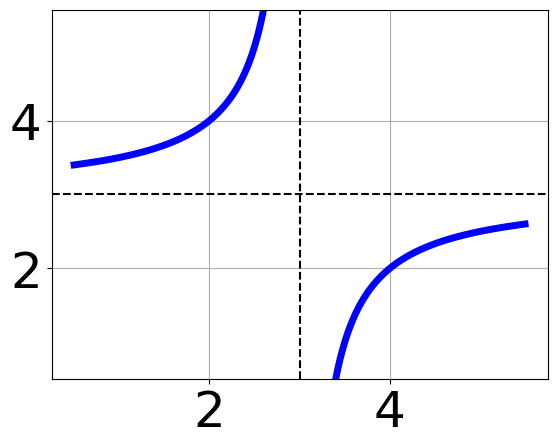
\includegraphics[width=0.3\textwidth]{../Figures/rationalEquationToGraphBB.png}
    \end{center}\begin{enumerate}[label=\Alph*.]
\begin{multicols}{2}
\item 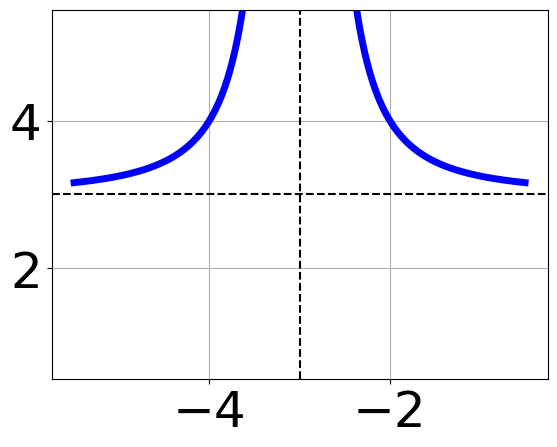
\includegraphics[width = 0.3\textwidth]{../Figures/rationalEquationToGraphAB.png}
\item 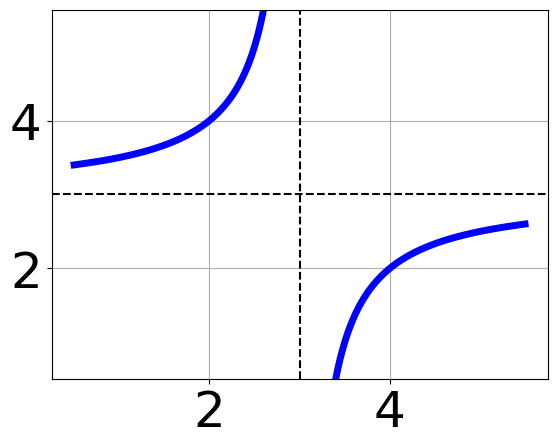
\includegraphics[width = 0.3\textwidth]{../Figures/rationalEquationToGraphBB.png}
\item 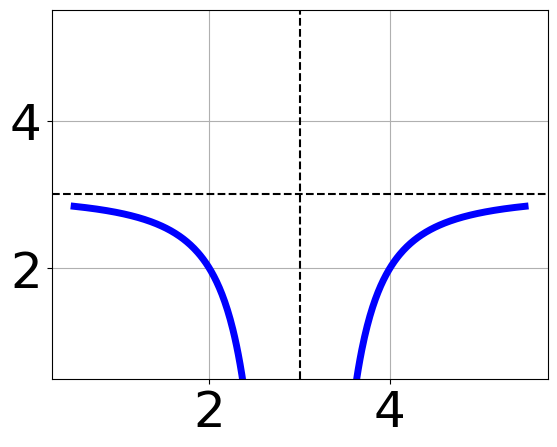
\includegraphics[width = 0.3\textwidth]{../Figures/rationalEquationToGraphCB.png}
\item 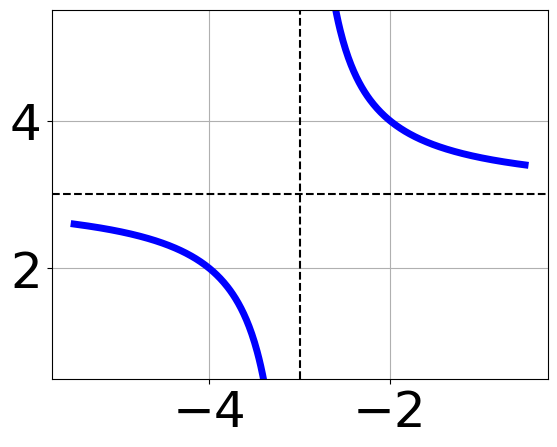
\includegraphics[width = 0.3\textwidth]{../Figures/rationalEquationToGraphDB.png}
\end{multicols}\item None of the above.\end{enumerate}
\textbf{General Comment:} Remember that the general form of a basic rational equation is $ f(x) = \frac{a}{(x-h)^n} + k$, where $a$ is the leading coefficient (and in this case, we assume is either $1$ or $-1$), $n$ is the degree (in this case, either $1$ or $2$), and $(h, k)$ is the intersection of the asymptotes.
}
\litem{
Solve the rational equation below. Then, choose the interval(s) that the solution(s) belongs to.
\[ \frac{98}{-42x + 70} + 1 = \frac{98}{-42x + 70} \]The solution is \( \text{all solutions are invalid or lead to complex values in the equation.} \), which is option C.\begin{enumerate}[label=\Alph*.]
\item \( x_1 \in [-2.67, 0.33] \text{ and } x_2 \in [-0.33,2.67] \)

$x = -1.667 \text{ and } x = 1.667$, which corresponds to getting the correct solution and believing there should be a second solution to the equation.
\item \( x \in [-2.67,0.33] \)

$x = -1.667$, which corresponds to not distributing the factor $-42x + 70$ correctly when trying to eliminate the fraction.
\item \( \text{All solutions lead to invalid or complex values in the equation.} \)

*$x = 1.667$ leads to dividing by 0 in the original equation and thus is not a valid solution, which is the correct option.
\item \( x \in [0.67,2.67] \)

$x = 1.667$, which corresponds to not checking if this value leads to dividing by 0 in the original equation and thus is not a valid solution.
\item \( x_1 \in [0.67, 2.67] \text{ and } x_2 \in [-0.33,2.67] \)

$x = 1.667 \text{ and } x = 1.667$, which corresponds to getting the correct solution and believing there should be a second solution to the equation.
\end{enumerate}

\textbf{General Comment:} Distractors are different based on the number of solutions. Remember that after solving, we need to make sure our solution does not make the original equation divide by zero!
}
\litem{
Choose the graph of the equation below.
\[ f(x) = \frac{1}{x - 1} - 1 \]The solution is the graph below, which is option A.
    \begin{center}
        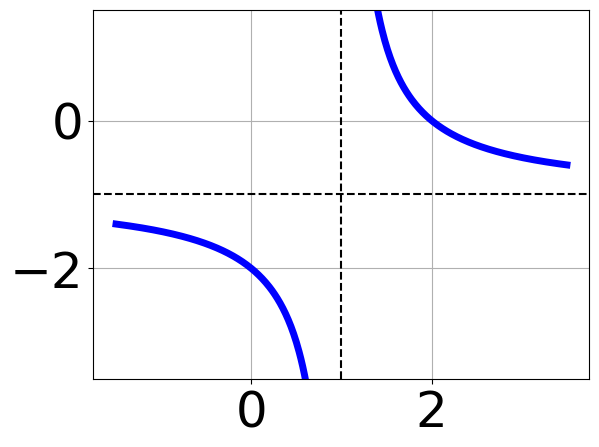
\includegraphics[width=0.3\textwidth]{../Figures/rationalEquationToGraphCopyAB.png}
    \end{center}\begin{enumerate}[label=\Alph*.]
\begin{multicols}{2}
\item 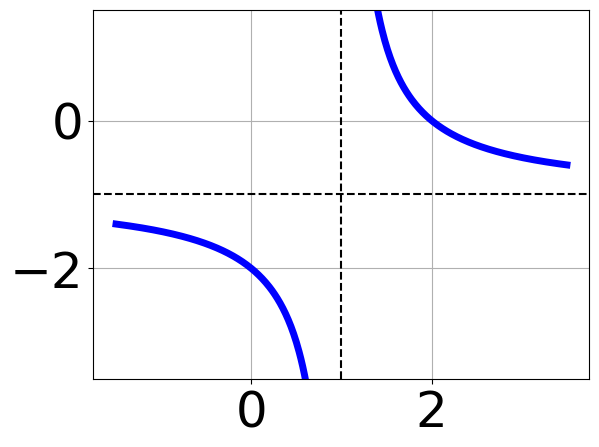
\includegraphics[width = 0.3\textwidth]{../Figures/rationalEquationToGraphCopyAB.png}
\item 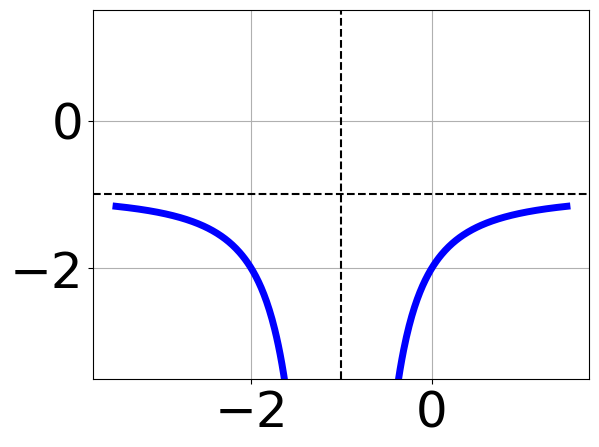
\includegraphics[width = 0.3\textwidth]{../Figures/rationalEquationToGraphCopyBB.png}
\item 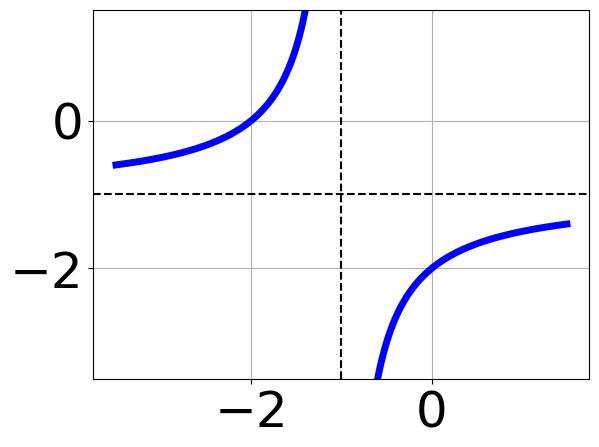
\includegraphics[width = 0.3\textwidth]{../Figures/rationalEquationToGraphCopyCB.png}
\item 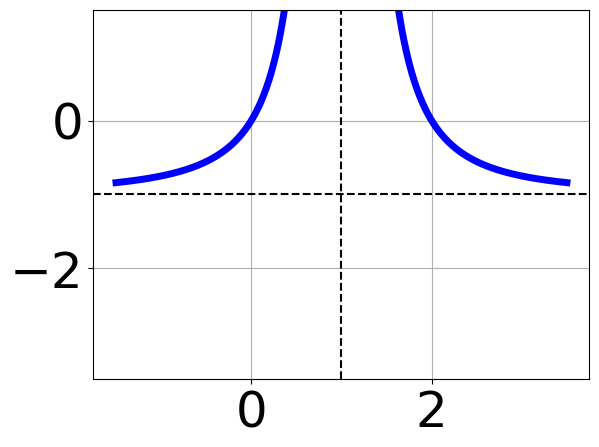
\includegraphics[width = 0.3\textwidth]{../Figures/rationalEquationToGraphCopyDB.png}
\end{multicols}\item None of the above.\end{enumerate}
\textbf{General Comment:} Remember that the general form of a basic rational equation is $ f(x) = \frac{a}{(x-h)^n} + k$, where $a$ is the leading coefficient (and in this case, we assume is either $1$ or $-1$), $n$ is the degree (in this case, either $1$ or $2$), and $(h, k)$ is the intersection of the asymptotes.
}
\litem{
Solve the rational equation below. Then, choose the interval(s) that the solution(s) belongs to.
\[ \frac{3}{-8x + 3} + -4 = \frac{9}{64x -24} \]The solution is \( x = 0.246 \), which is option B.\begin{enumerate}[label=\Alph*.]
\item \( \text{All solutions lead to invalid or complex values in the equation.} \)

This corresponds to thinking $x = 0.246$ leads to dividing by zero in the original equation, which it does not.
\item \( x \in [0.25,2.25] \)

* $x = 0.246$, which is the correct option.
\item \( x \in [-1.3,-0.2] \)

$x = -0.504$, which corresponds to not distributing the factor $-8x + 3$ correctly when trying to eliminate the fraction.
\item \( x_1 \in [-1.3, -0.2] \text{ and } x_2 \in [0.16,0.37] \)

$x = -0.504 \text{ and } x = 0.246$, which corresponds to getting the correct solution and believing there should be a second solution to the equation.
\item \( x_1 \in [0, 0.6] \text{ and } x_2 \in [0.49,0.57] \)

$x = 0.246 \text{ and } x = 0.562$, which corresponds to getting the correct solution and believing there should be a second solution to the equation.
\end{enumerate}

\textbf{General Comment:} Distractors are different based on the number of solutions. Remember that after solving, we need to make sure our solution does not make the original equation divide by zero!
}
\litem{
Determine the domain of the function below.
\[ f(x) = \frac{5}{18x^{2} -33 x + 15} \]The solution is \( \text{All Real numbers except } x = 0.833 \text{ and } x = 1.000. \), which is option E.\begin{enumerate}[label=\Alph*.]
\item \( \text{All Real numbers except } x = a, \text{ where } a \in [0.65, 0.85] \)

All Real numbers except $x = 0.833$, which corresponds to removing only 1 value from the denominator.
\item \( \text{All Real numbers except } x = a \text{ and } x = b, \text{ where } a \in [8.93, 9.23] \text{ and } b \in [29.76, 30.07] \)

All Real numbers except $x = 9.000$ and $x = 30.000$, which corresponds to not factoring the denominator correctly.
\item \( \text{All Real numbers.} \)

This corresponds to thinking the denominator has complex roots or that rational functions have a domain of all Real numbers.
\item \( \text{All Real numbers except } x = a, \text{ where } a \in [8.93, 9.23] \)

All Real numbers except $x = 9.000$, which corresponds to removing a distractor value from the denominator.
\item \( \text{All Real numbers except } x = a \text{ and } x = b, \text{ where } a \in [0.65, 0.85] \text{ and } b \in [0.85, 1.05] \)

All Real numbers except $x = 0.833$ and $x = 1.000$, which is the correct option.
\end{enumerate}

\textbf{General Comment:} Recall that dividing by zero is not a real number. Therefore the domain is all real numbers \textbf{except} those that make the denominator 0.
}
\litem{
Choose the equation of the function graphed below.

\begin{center}
    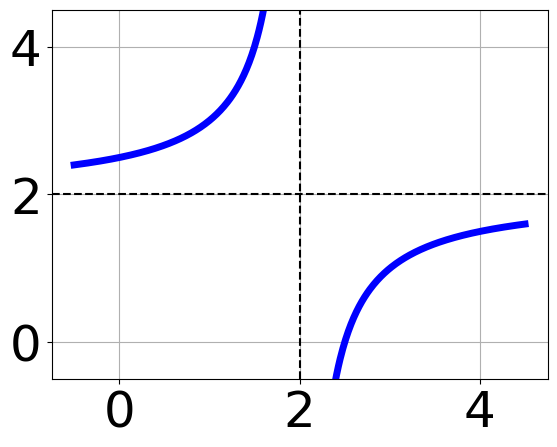
\includegraphics[width=0.5\textwidth]{../Figures/rationalGraphToEquationB.png}
\end{center}


The solution is \( \text{None of the above as it should be } f(x) = \frac{-1}{x - 2} + 2 \), which is option E.\begin{enumerate}[label=\Alph*.]
\item \( f(x) = \frac{1}{x - 2} + 0 \)

Corresponds to using the general form $f(x) = \frac{a}{x-h}+k$, the opposite leading coefficient AND not noticing the $y$-value was wrong.
\item \( f(x) = \frac{-1}{x + 2} + 0 \)

The $x$- and $y$-value of the equation does not match the graph.
\item \( f(x) = \frac{1}{(x - 2)^2} + 0 \)

Corresponds to thinking the graph was a shifted version of $\frac{1}{x^2}$, using the general form $f(x) = \frac{a}{x-h}+k$, the opposite leading coefficient, AND not noticing the $y$-value was wrong.
\item \( f(x) = \frac{-1}{(x + 2)^2} + 0 \)

Corresponds to thinking the graph was a shifted version of $\frac{1}{x^2}$ not noticing the $y$-value was wrong.
\item \( \text{None of the above} \)

None of the equation options were the correct equation.
\end{enumerate}

\textbf{General Comment:} Remember that the general form of a basic rational equation is $ f(x) = \frac{a}{(x-h)^n} + k$, where $a$ is the leading coefficient (and in this case, we assume is either $1$ or $-1$), $n$ is the degree (in this case, either $1$ or $2$), and $(h, k)$ is the intersection of the asymptotes.
}
\litem{
Determine the domain of the function below.
\[ f(x) = \frac{6}{9x^{2} +9 x -18} \]The solution is \( \text{All Real numbers except } x = -2.000 \text{ and } x = 1.000. \), which is option B.\begin{enumerate}[label=\Alph*.]
\item \( \text{All Real numbers.} \)

This corresponds to thinking the denominator has complex roots or that rational functions have a domain of all Real numbers.
\item \( \text{All Real numbers except } x = a \text{ and } x = b, \text{ where } a \in [-2.2, -1.9] \text{ and } b \in [0.5, 3.3] \)

All Real numbers except $x = -2.000$ and $x = 1.000$, which is the correct option.
\item \( \text{All Real numbers except } x = a, \text{ where } a \in [-2.2, -1.9] \)

All Real numbers except $x = -2.000$, which corresponds to removing only 1 value from the denominator.
\item \( \text{All Real numbers except } x = a \text{ and } x = b, \text{ where } a \in [-19.1, -16.9] \text{ and } b \in [8.3, 10.9] \)

All Real numbers except $x = -18.000$ and $x = 9.000$, which corresponds to not factoring the denominator correctly.
\item \( \text{All Real numbers except } x = a, \text{ where } a \in [-19.1, -16.9] \)

All Real numbers except $x = -18.000$, which corresponds to removing a distractor value from the denominator.
\end{enumerate}

\textbf{General Comment:} Recall that dividing by zero is not a real number. Therefore the domain is all real numbers \textbf{except} those that make the denominator 0.
}
\litem{
Choose the equation of the function graphed below.

\begin{center}
    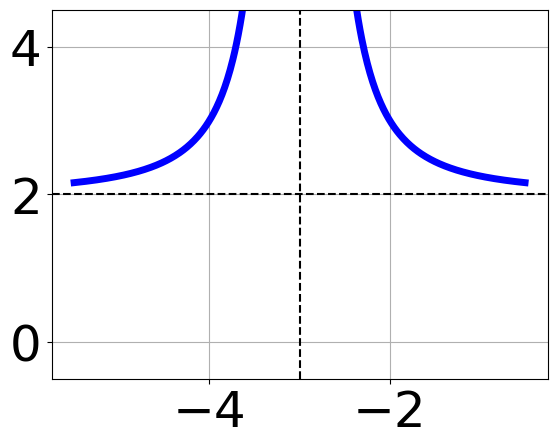
\includegraphics[width=0.5\textwidth]{../Figures/rationalGraphToEquationCopyB.png}
\end{center}


The solution is \( \text{None of the above as it should be } f(x) = \frac{1}{(x + 3)^2} + 2 \), which is option E.\begin{enumerate}[label=\Alph*.]
\item \( f(x) = \frac{-1}{x + 3} - 5 \)

Corresponds to thinking the graph was a shifted version of $\frac{1}{x}$, using the general form $f(x) = \frac{a}{(x-h)^2}+k$, the opposite leading coefficient, AND not noticing the $y$-value was wrong.
\item \( f(x) = \frac{-1}{(x + 3)^2} - 5 \)

Corresponds to using the general form $f(x) = \frac{a}{(x-h)^2}+k$, the opposite leading coefficient, AND not noticing the $y$-value was wrong.
\item \( f(x) = \frac{1}{x - 3} - 5 \)

Corresponds to thinking the graph was a shifted version of $\frac{1}{x}$ AND not noticing the $y$-value was wrong.
\item \( f(x) = \frac{1}{(x - 3)^2} - 5 \)

The $x$- and $y$-value of the equation does not match the graph.
\item \( \text{None of the above} \)

None of the equation options were the correct equation.
\end{enumerate}

\textbf{General Comment:} Remember that the general form of a basic rational equation is $ f(x) = \frac{a}{(x-h)^n} + k$, where $a$ is the leading coefficient (and in this case, we assume is either $1$ or $-1$), $n$ is the degree (in this case, either $1$ or $2$), and $(h, k)$ is the intersection of the asymptotes.
}
\litem{
Solve the rational equation below. Then, choose the interval(s) that the solution(s) belongs to.
\[ \frac{6x}{-5x -4} + \frac{-7x^{2}}{-30x^{2} -49 x -20} = \frac{-2}{6x + 5} \]The solution is \( \text{There are two solutions: } x = 0.283 \text{ and } x = -0.973 \), which is option B.\begin{enumerate}[label=\Alph*.]
\item \( x \in [-1.07,-0.97] \)


\item \( x_1 \in [0.09, 0.72] \text{ and } x_2 \in [-1.6,-0.81] \)

* $x = 0.283 \text{ and } x = -0.973$, which is the correct option.
\item \( x_1 \in [0.09, 0.72] \text{ and } x_2 \in [-0.82,-0.29] \)


\item \( x \in [-0.88,-0.27] \)


\item \( \text{All solutions lead to invalid or complex values in the equation.} \)


\end{enumerate}

\textbf{General Comment:} Distractors are different based on the number of solutions. Remember that after solving, we need to make sure our solution does not make the original equation divide by zero!
}
\litem{
Solve the rational equation below. Then, choose the interval(s) that the solution(s) belongs to.
\[ \frac{2x}{4x + 4} + \frac{-6x^{2}}{-16x^{2} -40 x -24} = \frac{7}{-4x -6} \]The solution is \( \text{There are two solutions: } x = -1.631 \text{ and } x = -1.227 \), which is option A.\begin{enumerate}[label=\Alph*.]
\item \( x_1 \in [-1.73, -1.62] \text{ and } x_2 \in [-1.39,-1.19] \)

* $x = -1.631 \text{ and } x = -1.227$, which is the correct option.
\item \( x \in [-1.37,-1.19] \)


\item \( x_1 \in [-1.73, -1.62] \text{ and } x_2 \in [-1.17,-0.52] \)


\item \( \text{All solutions lead to invalid or complex values in the equation.} \)


\item \( x \in [-1.58,-1.47] \)


\end{enumerate}

\textbf{General Comment:} Distractors are different based on the number of solutions. Remember that after solving, we need to make sure our solution does not make the original equation divide by zero!
}
\end{enumerate}

\end{document}